%-------------------------------------------------------------------------------------------------------------
%       P A R Á M E T R O S   D E   C O M P I L A C I Ó N
%--------------------------------------------------------------
% PDFLaTeX --> BibTeX (x2) --> PDFLaTeX (x2) --> Ver PDF
%--------------------------------------------------------------------------------------------------------------
%                 R E C O M E N D A C I O N E S
%----------------------------------------------------------
% SE RECOMIENDA AMPLIAMENTE NO EDITAR EL DOCUMENTO "example.sty" o "portadaposgradoMCM.sty" QUE CONTIENE LAS CONDICIONES Y ESPECIFICACIONES PROPUESTAS POR EL DEPARTAMENTO
% EL DOCUMENTO "biblio.bib" CONTIENE LA BIBLIOGRAFÍA CON UN PAR DE EJEMPLOS
%--------------------------------------------------------------------------------------------------------------
%                A J U S T E S   D E   I N I C I O 
%--------------------------------------------------------------------------------------------------------------
\PassOptionsToPackage{usenames,dvipsnames}{color}% NO EDITAR 
\documentclass[letterpaper,openright,12pt, oneside, spanish]{book}% NO EDITAR 
\usepackage{example}% NO EDITAR 
\usepackage{portada_oficial_itm}% NO EDITAR
%----------------------------------------------------------
%                D A T O S   P O R T A D A
%----------------------------------------------------------
\DeclareLanguageMapping{spanish}{spanish-apa}
\addbibresource{bibliografia.bib}
\author{Br. Giovanny González Baltazar}%EDITAR
\title{Arquitectura para control inteligente de tráfico urbano}%EDITAR
\institucion{instituto tecnológico de mérida}%NO EDITAR
\departamento{división de estudios profesionales}%NO EDITAR
\programa{departamento de sistemas}%EDITAR
\grado{ingeniero(a)}%EDITAR
\asesor{Dr. Joel Antonio Trejo Sánchez}
\coasesor{Dr. Mauricio Gabriel Orozco del Castillo}
%--------------------------------------------------------------------------------------------------------------
%                        D O C U M E N T O
%--------------------------------------------------------------------------------------------------------------
\begin{document}  
%--------------------------------------------------------------------------------------------------------------
%                 C U E R P O   P R E L I M I N A R
%--------------------------------------------------------------------------------------------------------------
\pagenumbering{Roman} % Númeración Romana		
\maketitle % Compila parametros de la portada
\newpage % Nueva página
\afterpage{\blankpage}
%\includepdf[pages=-]{Adjuntos/firmas.pdf} %  Firmas de impresión definitiva
\chapter*{Dedicatoria} % si no queremos que añada la palabra "Capitulo"
\addcontentsline{toc}{chapter}{Dedicatoria} % si queremos que aparezca en el Í­ndice
\markboth{Dedicatoria}{Dedicatoria} % encabezado

\linespread{1.3}
{\Huge{(\textit{Página de dedicatoria})}}
\clearpage % Incluye la dedicatoria
\chapter*{Agradecimientos} % si no queremos que añada la palabra "Capitulo"
\addcontentsline{toc}{chapter}{Agradecimientos} % si queremos que aparezca en el Í­ndice
\markboth{Agradecimientos}{Agradecimientos} % encabezado
\linespread{1.3}
{\Huge{(\textit{Página de agradecimientos})}}
\clearpage % Start a new page % Incluye los agradecimientos
\setcounter{page}{1} % Empieza la numeración Romana
\chapter*{Resumen} % si no queremos que añada la palabra "Capitulo"
\addcontentsline{toc}{chapter}{Resumen} % si queremos que aparezca en el Í­ndice
\markboth{RESUMEN}{RESUMEN} % encabezado
\noindent \rule{0.9\textwidth}{1.0pt} \newline
\noindent \textbf{\textit{Palabras clave}: }\newline
\noindent \rule{0.9\textwidth}{1.0pt}
\ \newline
\par
\linespread{1.3}
{\Huge{(\textit{Página de resumen})}}
\clearpage % Nueva página


% TODO: Como mi trabajo amplía al del Dr. y al del otro chavo, citarlos aquí en la intro % Incluye resumen
\chapter*{Abstract} % si no queremos que añada la palabra "Capitulo"
\addcontentsline{toc}{chapter}{Abstract} % si queremos que aparezca en el Í­ndice
\markboth{ABSTRACT}{ABSTRACT} % encabezado
\noindent \rule{0.9\textwidth}{1.0pt} \newline
\noindent \textbf{\textit{Keywords}:} \newline
\noindent \rule{0.9\textwidth}{1.0pt}
\ \newline
\par
\linespread{1.3}
{\Huge{(\textit{Abstract page})}}
\clearpage % Nueva página
 % Incluye abstract
\newpage
\tableofcontents %  Crea índice
\newpage
\listoftables % Lista de Tablas
\newpage
\listoffigures % Lista de Figuras
\newpage
\input{Adjuntos/borrador_Nomenclatura} % Incluye nomenclatura
\newpage
%---------------------------------------------------------------------------------------------------------------
%                 C U E R P O   P R I N C I P A L
%---------------------------------------------------------------------------------------------------------------
\pagenumbering{arabic} %Numeración Arábiga
\setcounter{page}{1}
\clearpage
\newpage
\thispagestyle{empty}
\vspace*{\fill}
\begingroup
\centering
\begin{flushright}{\fontsize{50}{60}\selectfont CAPÍTULO 1}\end{flushright}
\vspace{10 mm}
\begin{flushright}{\fontsize{30}{40}\selectfont INTRODUCCIÓN }\end{flushright}
\endgroup
\vspace*{\fill}
\newpage
\input{Capitulos/borrador_cap_1}
\clearpage
% \newpage
\thispagestyle{empty}
\vspace*{\fill}
\begingroup
\centering
\begin{flushright}{\fontsize{50}{60}\selectfont CAPÍTULO 2}\end{flushright}
\vspace{10 mm}
\begin{flushright}{\fontsize{30}{40}\selectfont MARCO TEÓRICO }\end{flushright}
\endgroup
\vspace*{\fill}
\newpage
% \chapter{Marco Teórico} % con la palabra capitulo
%\addcontentsline{toc}{chapter}{Capítulo 2: Marco Teórico} % si queremos que aparezca en el Í­ndice
%\markboth{Capítulo 2: Marco Teórico}{Capítulo 2: Marco Teórico} % encabezado
\graphicspath{./imagenes}

En éste capítulo se muestra un ejemplo de un diagrama en la Figura \ref{fig:diagrama}
\begin{figure}[hbtp]
\scalebox{0.6}{\input{diagramas/ejemplo_diagrama.tex}}
\caption{Ejemplo de diagrama.}
\label{fig:diagrama}
\end{figure}
\clearpage%


% \clearpage
% \newpage
\thispagestyle{empty}
\vspace*{\fill}
\begingroup
\centering
\begin{flushright}{\fontsize{50}{60}\selectfont CAPÍTULO 3}\end{flushright}
\vspace{10 mm}
\begin{flushright}{\fontsize{30}{40}\selectfont METODOLOGÍA }\end{flushright}
\endgroup
\vspace*{\fill}
\newpage
% \chapter{Metodología}\label{cap3} % con la palabra capitulo
%\addcontentsline{toc}{chapter}{Capítulo 2: Marco Teórico} % si queremos que aparezca en el Í­ndice
%\markboth{Capítulo 2: Marco Teórico}{Capítulo 2: Marco Teórico} % encabezado
\graphicspath{./imagenes}
En la Figura \ref{fig:ejem1} se muestra una imagen de ejemplo 
\begin{figure}[hbtp]
\centering
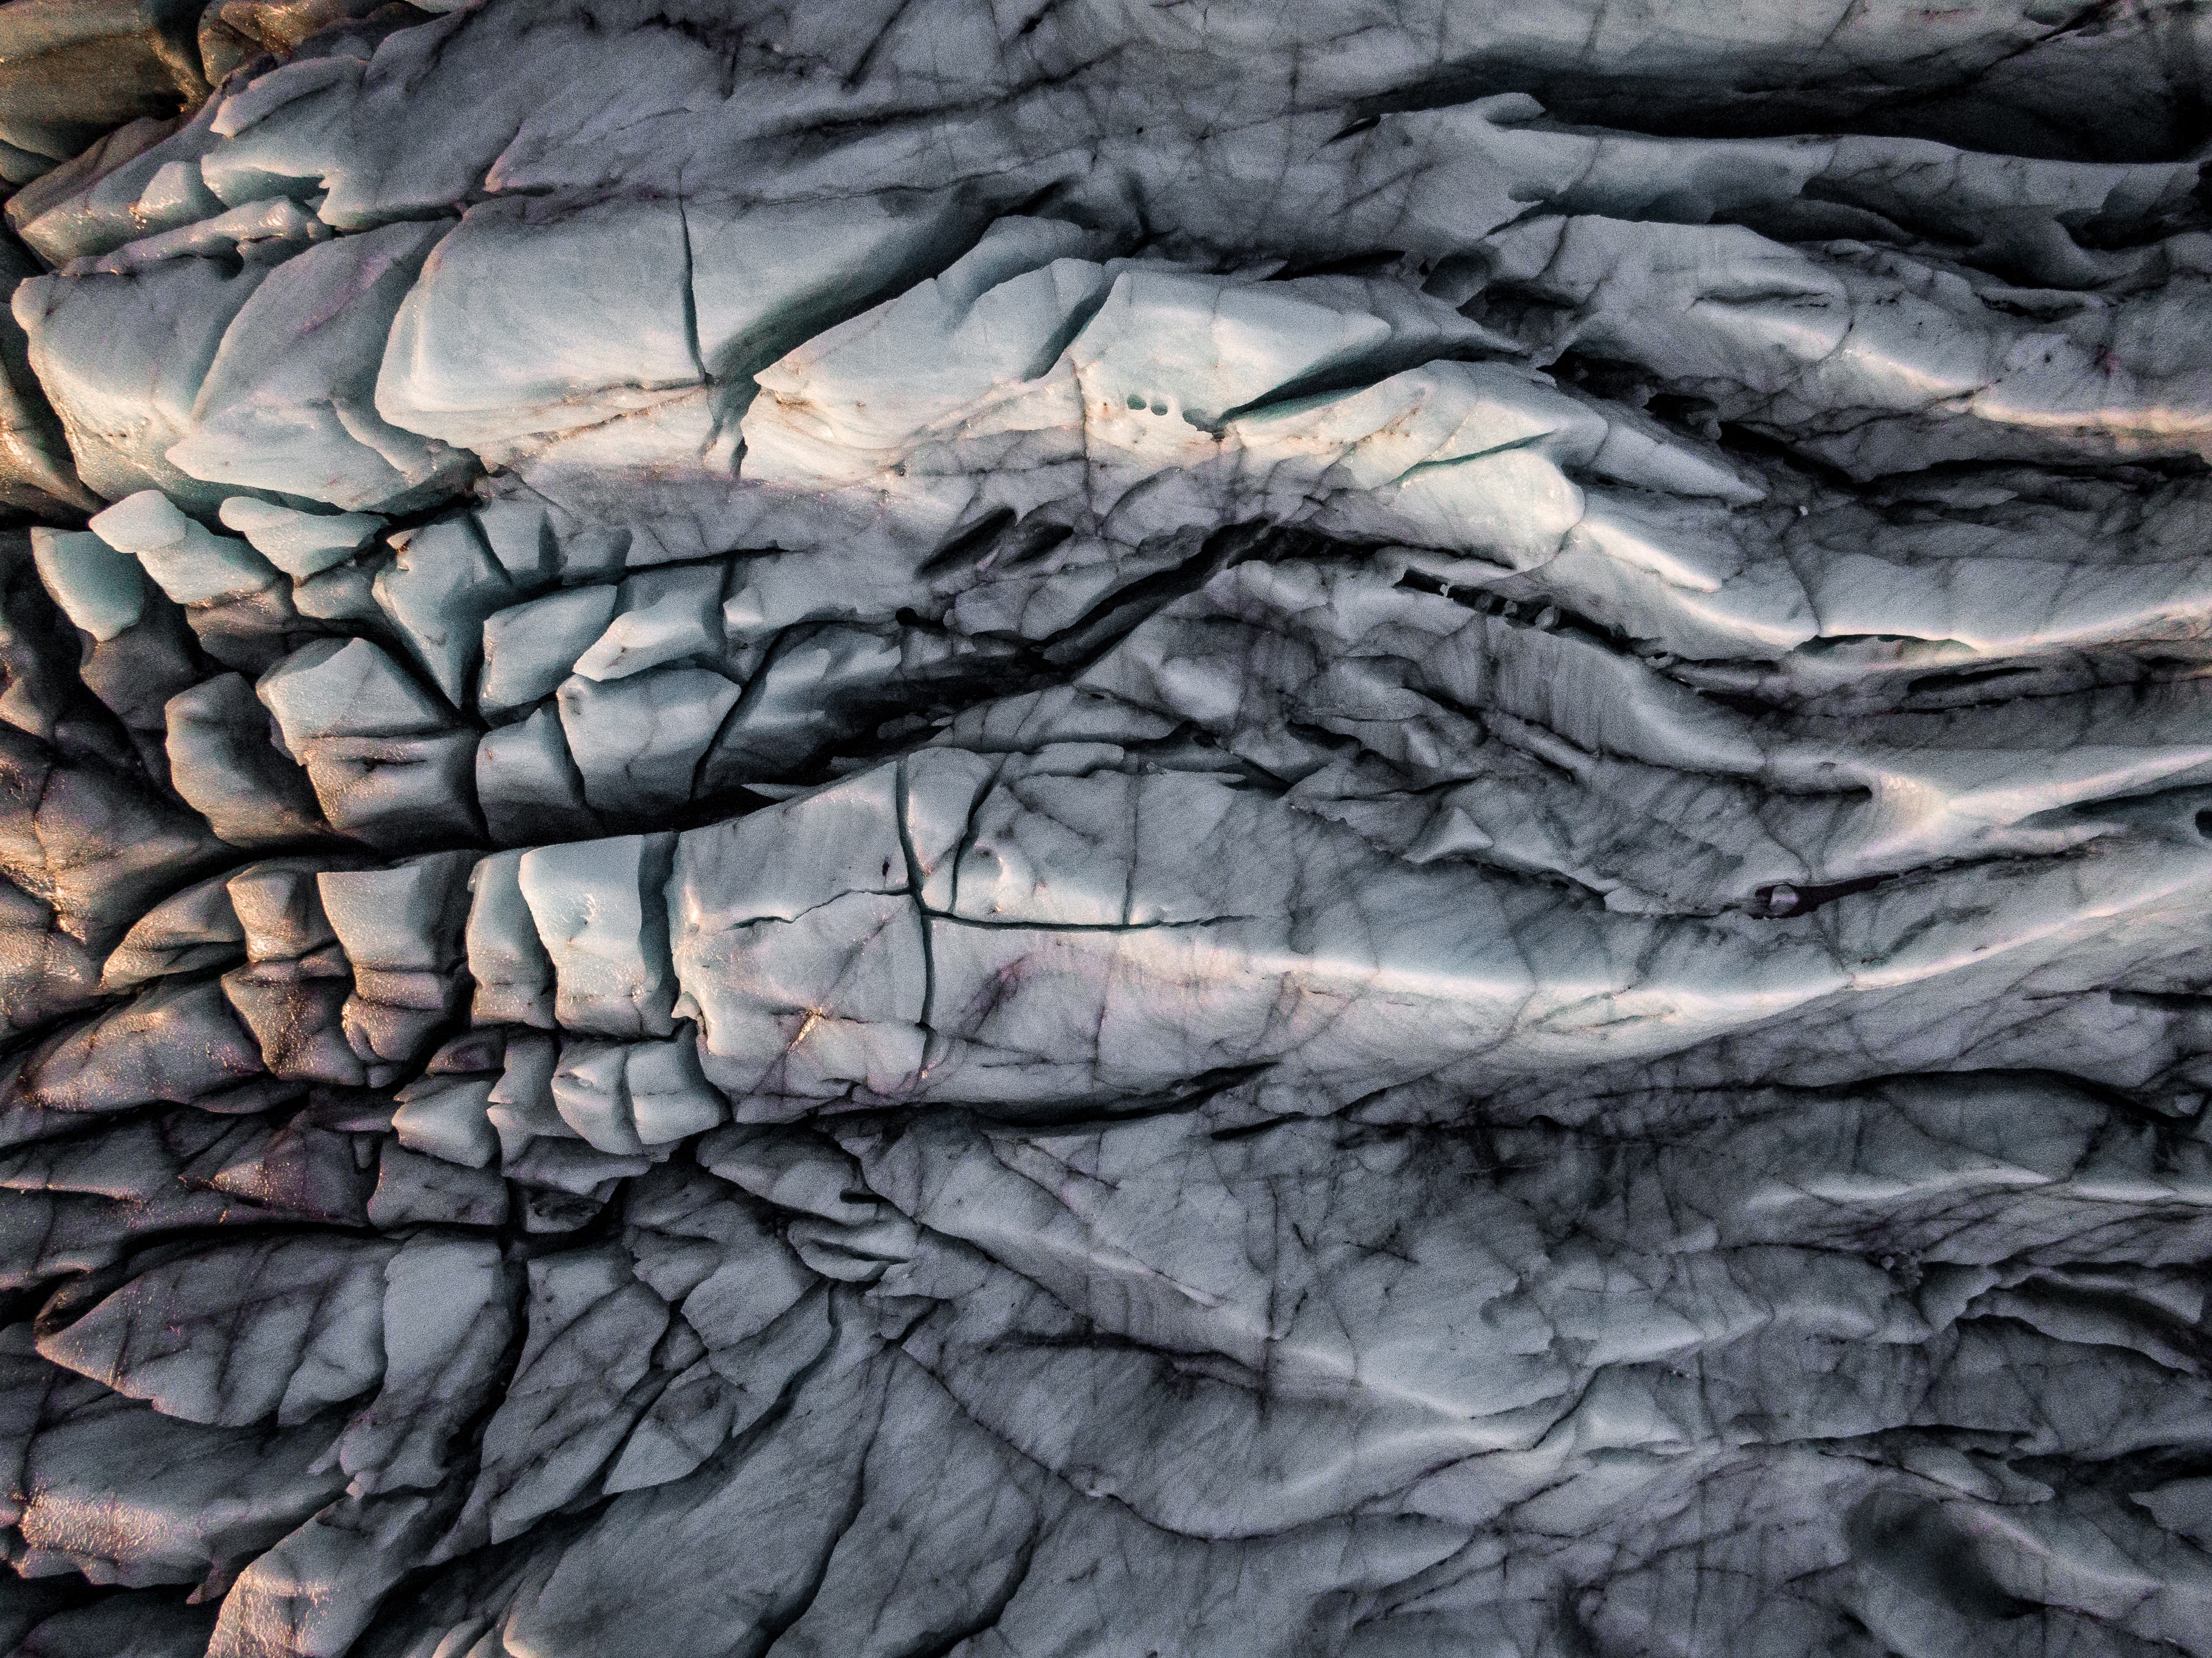
\includegraphics[scale=0.1]{imagenes/tomas.jpg}
\caption{Photo by Tomáš Malík on \href{https://unsplash.com/}{Unsplash}}
\label{fig:ejem1}
\end{figure}
\clearpage
En la Figura \ref{fig:ejem:2} se muestra un ejemplo de multiples figuras en una sola.
\begin{figure}[hbtp]
\centering
\subfigure[Photo by dylan nolte on \href{https://unsplash.com/}{Unsplash}]{
\includegraphics[scale=0.03]{imagenes/dylan.jpg}}
\subfigure[Photo by Kai Dahms on \href{https://unsplash.com/}{Unsplash}]{\includegraphics[scale=0.03]{imagenes/kai.jpg}}\\
\subfigure[Photo by Raul Angel on \href{https://unsplash.com/}{Unsplash}]{\includegraphics[scale=0.056]{imagenes/raul.jpg}}
\subfigure[Photo by Stéphane Mingot on \href{https://unsplash.com/}{Unsplash}]{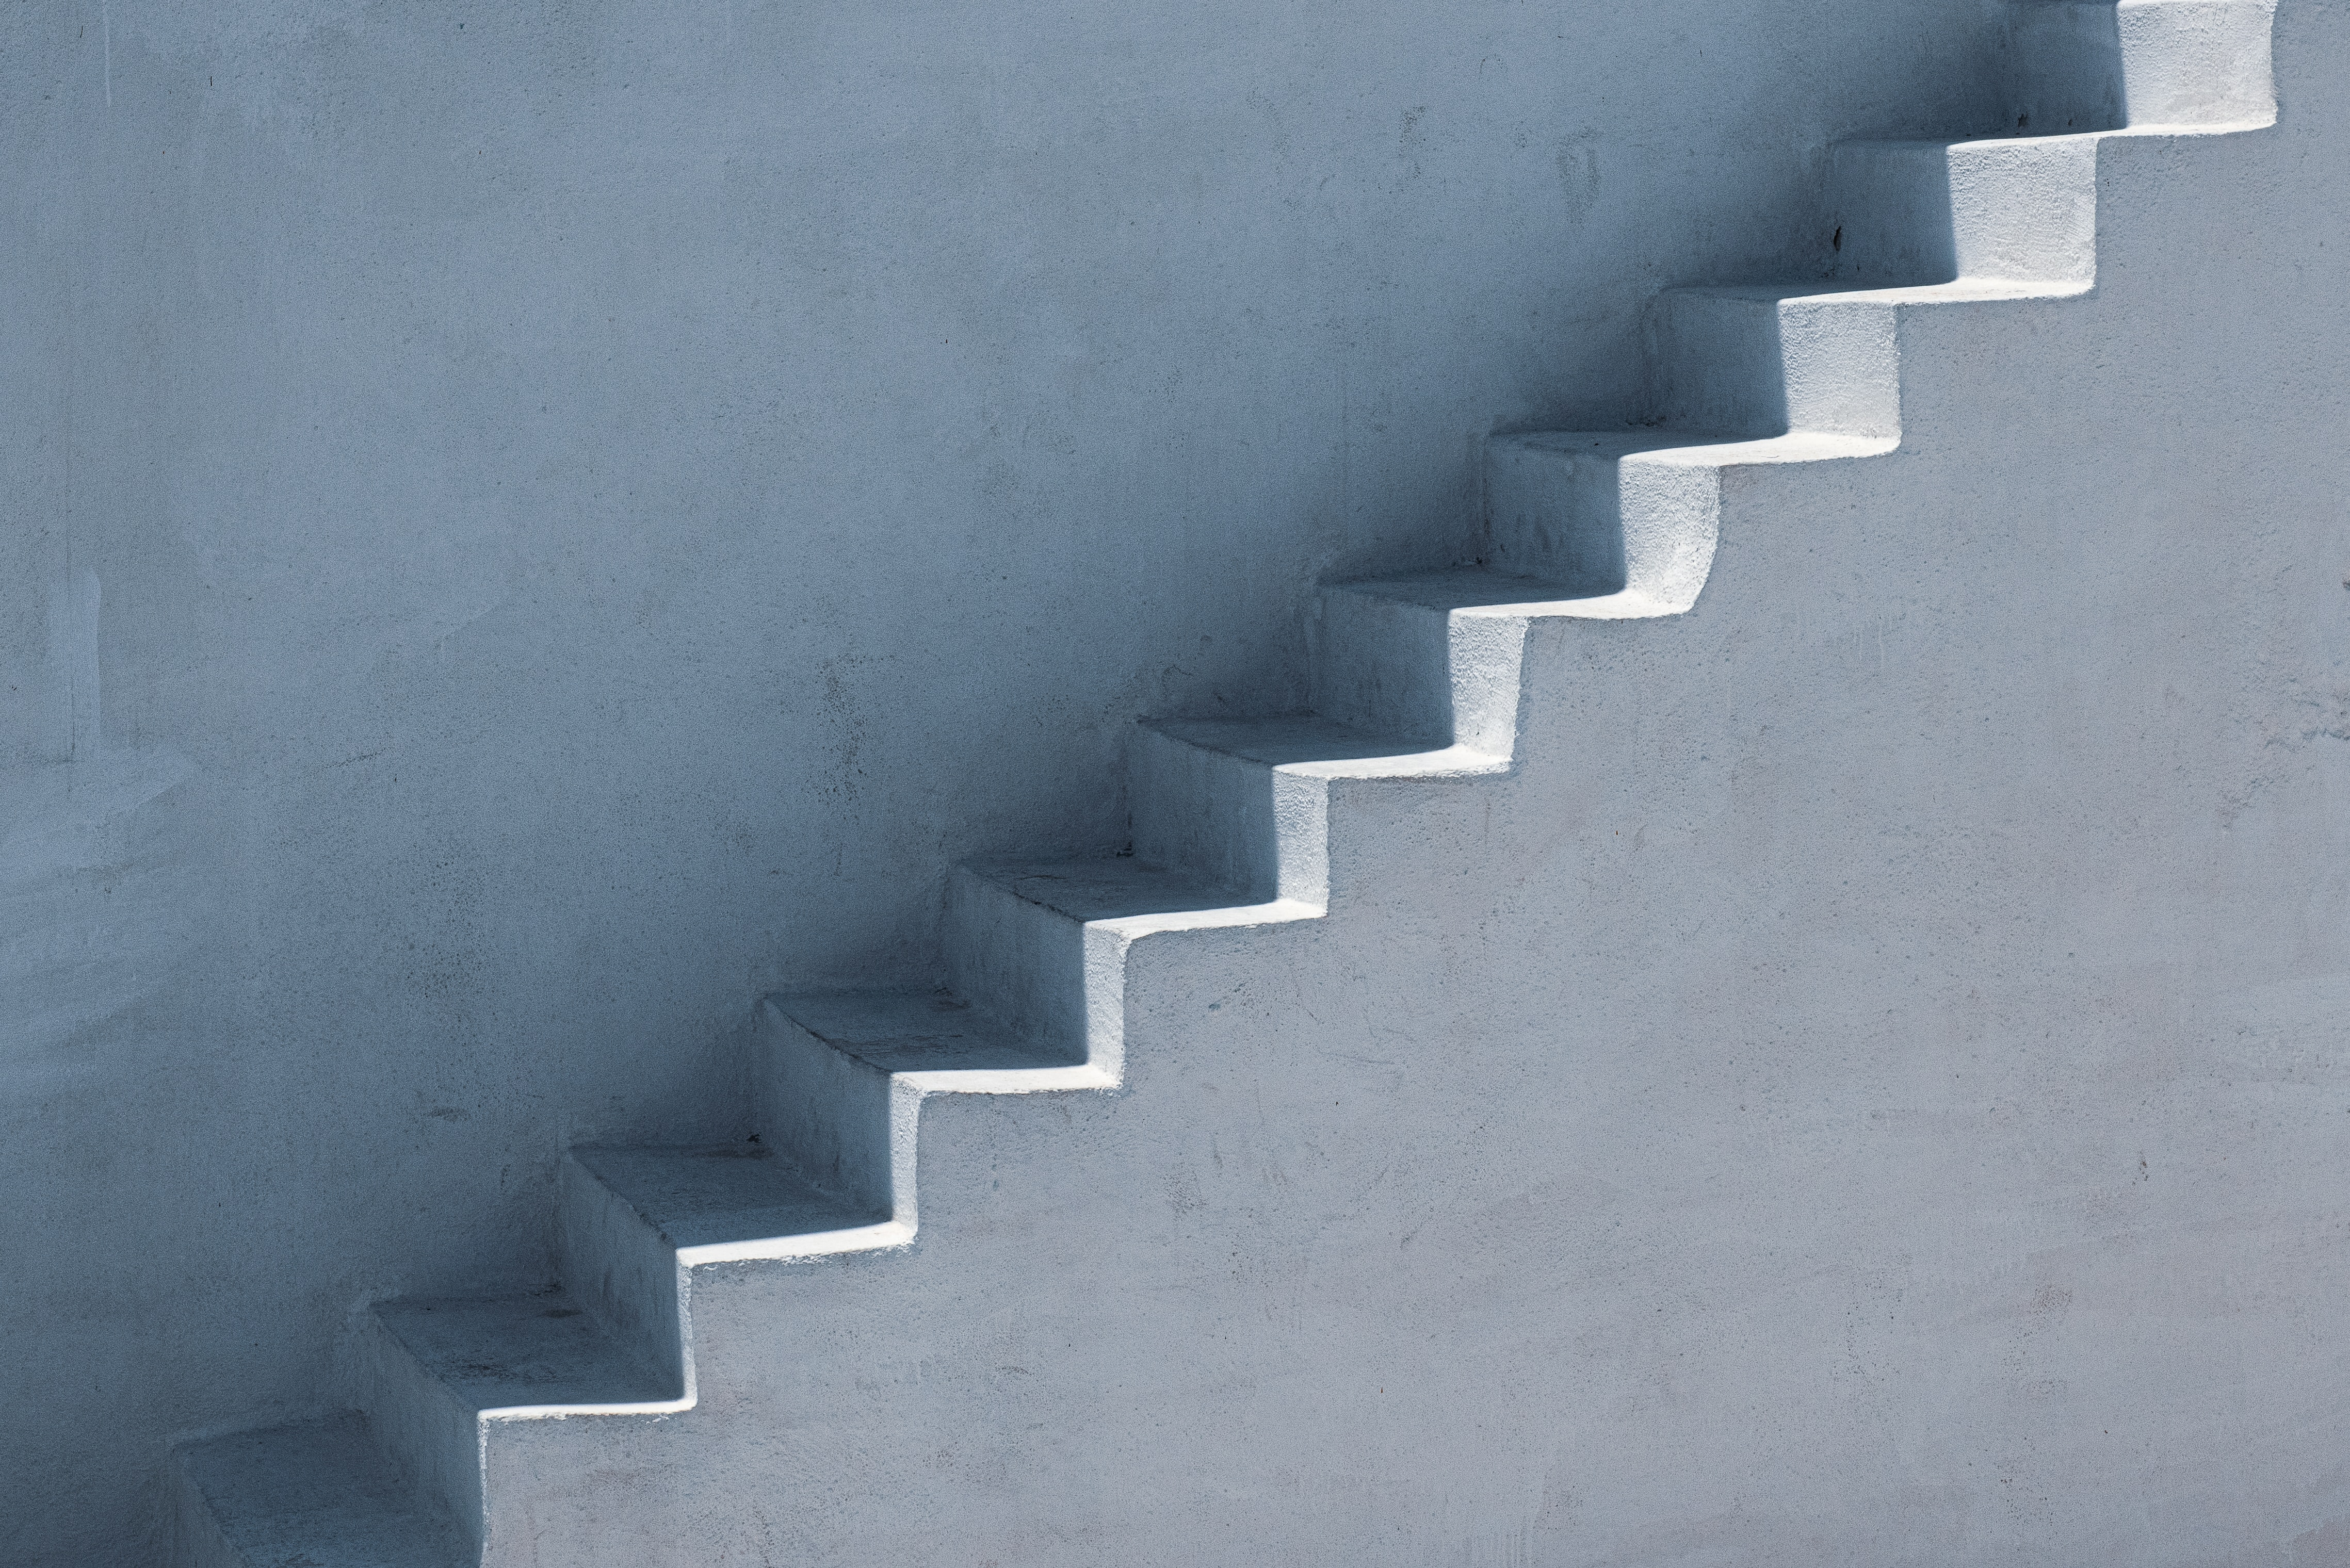
\includegraphics[scale=0.04]{imagenes/stephane.jpg}}\\
\caption{Ejemplo de ambiente Figure con múltiples imágenes}
\label{fig:ejem:2}
\end{figure}

La Tabla \ref{tab:ejem1} es un ejemplo para el estudiante sobre como construir tablas

\begin{table}[h]
\caption{Ejemplo de tabla.}
\begin{center}
\begin{tabular}{ cccc } 
\hline
col1 & col2 & col3 \\
\hline
\multirow{3}{4em}{Multiple row} & cell2 & cell3 \\ 
& cell5 & cell6 \\ 
& cell8 & cell9 \\ 
\hline
\end{tabular}
\label{tab:ejem1}
\end{center}
\end{table}


\clearpage%
% \clearpage
% \newpage
\thispagestyle{empty}
\vspace*{\fill}
\begingroup
\centering
\begin{flushright}{\fontsize{50}{60}\selectfont CAPÍTULO 4}\end{flushright}
\vspace{10 mm}
\begin{flushright}{\fontsize{30}{40}\selectfont RESULTADOS }\end{flushright}
\endgroup
\vspace*{\fill}
\newpage
% \chapter{Resultados}\label{cap4} % con la palabra capitulo
\graphicspath{{./graficas}}
%\addcontentsline{toc}{chapter}{Capítulo 2: Marco Teórico} % si queremos que aparezca en el Í­ndice
%\markboth{Capítulo 2: Marco Teórico}{Capítulo 2: Marco Teórico} % encabezado
\linespread{1.3}
En la Figura \ref{fig:graf} se muestra un ejemplo de una grafica añadida en formado .pdf (puede utilizarse formato .jpg, .png o directamente desde software graficador en formato .tex)
\begin{figure}[hbtp]
\centering
\includegraphics[scale=1]{/pg.pdf}
\caption{ejemplo de gráfica.}
\label{fig:graf}
\end{figure}
\clearpage%
\clearpage
\newpage
\thispagestyle{empty}
\vspace*{\fill}
\begingroup
\centering
\begin{flushright}{\fontsize{30}{40}\selectfont CONCLUSIONES}\end{flushright}
\endgroup
\vspace*{\fill}
\newpage
\chapter*{Conclusiones} % si no queremos que añada la palabra "Capitulo"
\addcontentsline{toc}{chapter}{Conclusiones} % si queremos que aparezca en el Í­ndice
\markboth{CONCLUSIONES}{CONCLUSIONES} % encabezado

\linespread{1.3}

\clearpage % Nueva página
\clearpage
%-----------------------------------------------------------------------------------------------------------------
%         B I B L I O G R A F I A   Y   A P E N D I C E S
%-----------------------------------------------------------------------------------------------------------------
\printbibliography[title={Referencias},heading=bibintoc]
\clearpage 
\newpage
\thispagestyle{empty}
\vspace*{\fill}
\begingroup
\centering
\begin{flushright}{\fontsize{30}{40}\selectfont APÉNDICE}\end{flushright}
\endgroup
\vspace*{\fill}
\newpage
\chapter*{Apéndice A} % si no queremos que añada la palabra "Capitulo"
\addcontentsline{toc}{chapter}{Apéndice A} % si queremos que aparezca en el Í­ndice
\markboth{Ap\'endice A}{Ap\'endice A} % encabezado

\linespread{1.3}

\noindent \textbf{\large{Software Utilizado}}
\ \newline
\par

En el presente trabajo se usaron los siguientes programas.

\begin{itemize}
	\item Programa 1
	\item Programa 2
	\item Programa 3
	\item Programa 4
	
\end{itemize}

Este trabajo ha sido escrito completamente en  \LaTeX usando el editor de texto Visual Studio Code con la extensión LaTeX Workshop desde archivos fuente en Markdown convertidos con Pandoc.
\clearpage % Nueva página




% \begin{versionhistory} 
% \begin{center}
%  \textbf{\docTitle}\\
%  \textbf{\vhListAllAuthors}\\
%  \textbf{Version} \vhCurrentVersion\ \\
% Fecha \vhCurrentDate
% \end{center} 
%  \vhEntry{1.0}{03.01.19}{MHO}{creado}
%  \vhEntry{1.1}{03.01.19}{JARB|CABH}{correcci\'{o}n}
%  \vhEntry{1.2}{05.01.19}{JARB|CABH}{revisado después de correcci\'{o}n}
% \end{versionhistory}
\clearpage % Incluye el apéndice
%-----------------------------------------------------------------------
\end{document}%